\documentclass[letterpaper,12pt]{article}
\usepackage[english]{babel}
\usepackage[utf8x]{inputenc}
\usepackage{amsmath}
\usepackage[paper=letterpaper,left=25mm,right=25mm,top=25mm,bottom=25mm]{geometry}
\usepackage{graphicx}
\usepackage[colorinlistoftodos]{todonotes}
\usepackage{newtxtext,newtxmath}
\usepackage{pgfplots}

\begin{document}
	
	\begin{titlepage}
		
		\newcommand{\HRule}{\rule{\linewidth}{0.5mm}}
		
		\center
		
		\textsc{\LARGE University of British Columbia}\\[1.5cm]
		\textsc{\Large MECH 325 - Mechanical Design I}\\[0.5cm]
		\textsc{\Large Assignment 1}\\[0.5cm]
		
		\HRule \\[0.8cm]
		{ \huge \bfseries Gear Train Design}\\[0.4cm]
		\HRule \\[1cm]
		
		{\Large GROUP C2}\\
		\vspace{0.5cm}
		
		\begin{minipage}{0.4\textwidth}
			\begin{flushleft} \large
				\emph{Team Member:}\\
				Kota Chang\\
				Chuan Du\\
				Donney Fan\\
				Dvir Hilu\\
				Michael Ko\\
				Priyansh Malik\\
				Darren Tong\\
			\end{flushleft}
		\end{minipage}
		~
		\begin{minipage}{0.4\textwidth}
			\begin{flushright} \large
				\emph{Student Number:} \\
				12345678\\
				12345678\\
				12345678\\
				12345678\\
				12345678\\
				12345678\\
				12345678
			\end{flushright}
		\end{minipage}\\[2cm]
		
		{\large \today}\\[2cm]
		
		{\large
			Velocity = 12345 mm/sec\\
			Cost = \$1245\\
			Performance Metric = 12345 mm/\$s
		}
		
		%\includegraphics{logo.png}\\[1cm]
		
		\vfill % Fill the rest of the page with whitespace
		
	\end{titlepage}
	
	\section{Summary}
	
	\newpage
	
	\section{Appendix}
	
	\subsection{Power Screw Analysis}
	
	The objective of this section is to find the minimum required torque and rotational speed needed to lift the 2500 kg load at 4 mm/sec.
	
	The torque required to lift a load with gravitational force $F$ is:
	
	\begin{equation}
	\tau = \frac{Fd_m}{2}\left(\frac{l+\pi f d_m}{\pi d_m - fl}\right)
	\end{equation}
	
	\begin{center}
		\begin{tabular}{ |p{2cm}||p{3cm}|p{2cm}|p{7cm}|  }
			\hline
			\multicolumn{4}{|c|}{Parameters} \\
			\hline
			Symbol& Value & Units & Description\\
			\hline
			$F$ & $2500 \times 9.81$ & N & Axial compressive force\\
			$d_m$ & 57 & mm   & Mean diameter\\
			$l$ & 6 & mm &  Pitch\\
			$f$ & 0.08 & N/A & Friction Coefficient\\
			\hline
		\end{tabular}
	\end{center}
	
A torque of 79.5 Nm is required to lift the load where efficiency losses in the power screw is accounted for by the friction coefficient, $f$. 

\subsection{Worm Gear Efficiency Analysis}
Worm gears are used in high torque applications but they are subject to efficiency losses during operation. Calculating this value allows us to find the gear train required to raise the load. \\

	\begin{equation}
	\eta = \frac{cos\phi_n - ftan\lambda}{cos\phi_n+fcot\lambda}
	\end{equation}
	
The helix angle component is as follows:

	\begin{equation}
\tan \lambda =  \frac{p_x}{\pi d_p} = 0.4074366
	\end{equation}

\begin{center}
		\begin{tabular}{ |p{2cm}||p{3cm}|p{2cm}|p{7cm}|  }
			\hline
			\multicolumn{4}{|c|}{Parameters} \\
			\hline
			Symbol& Value & Units & Description\\
			\hline
			$N_G$ & $18$ & N/A & Number of teeth on worm drive gear\\
			$N_w$ & 2 & N/A   & 2-thread worm \\
			$\phi_n$ & 14.5 & degrees &  Pressure angle\\
			$l$ & 16 & mm & pitch\\
			$p_x$ & 32 & mm & Axial pitch\\
			$d_p$ & 25 & mm & Worm pitch diameter\\
			$d_s$ & 20 & mm & Worm shaft diameter\\
			\hline
		\end{tabular}
	\end{center}


\subsection{Motor Torque Analysis}
The motor provided has the following torque-speed curve. The maximum power output occurs when the motor operates at 2500 rmp with 2.5 Nm of torque. \\

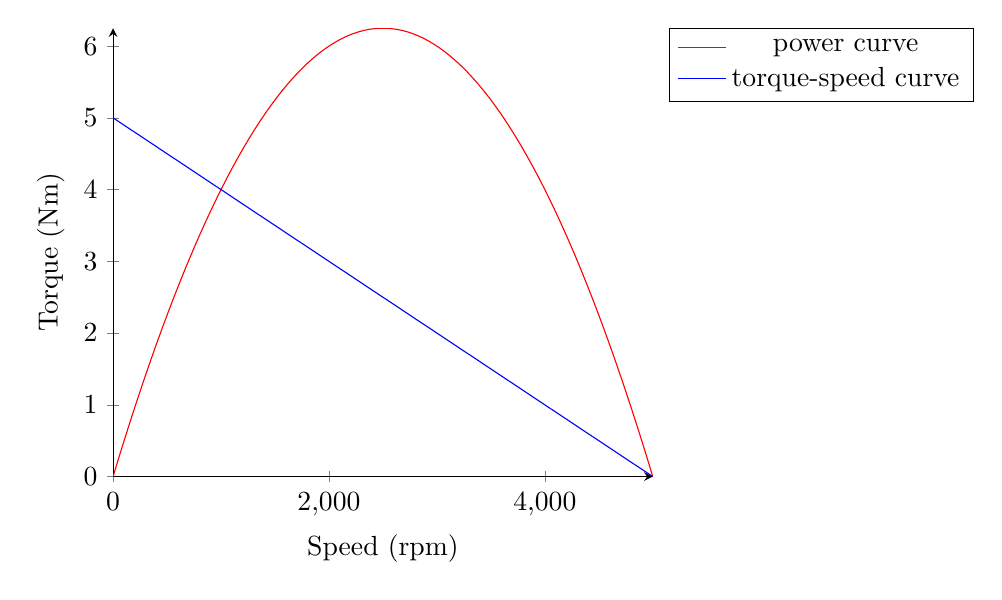
\begin{tikzpicture}
\begin{axis}[
    axis lines = left,
    xlabel = Speed (rpm),
    ylabel = {Torque (Nm)},
    xtick={0,2000,4000},
    ytick = {0,1,2,3,4,5,6,7},
    legend pos = outer north east
]
%Below the red parabola is defined
\addplot [
    domain=0:5000, 
    samples=100, 
    color=red,
]
{(-x^2/1000.0+5*x)/1000.0};
\addlegendentry{power curve}
\addplot [
    domain=0:5000, 
    samples=100, 
    color=blue,
    ]
    {-x/1000.0+5};
\addlegendentry{torque-speed curve}
 
\end{axis}
\end{tikzpicture}

\end{document}
